% !TEX encoding = UTF-8 Unicode
\documentclass{beamer}

\usepackage{cmap}
\usepackage[parfill]{parskip}
\usepackage{polyglossia}

% Related to math
\usepackage{amsmath,amssymb}
\usepackage{graphicx}
\usepackage{subcaption}

\setdefaultlanguage[spelling=modern]{russian}
\setotherlanguage{english}
\setmainfont{FreeSans}
\setsansfont{FreeSerif}
\setmonofont{FreeMono}

\addtobeamertemplate{navigation symbols}{}{%
    \usebeamerfont{footline}%
    \usebeamercolor[fg]{footline}%
    \hspace{1em}%
    \insertframenumber/\inserttotalframenumber
}


\title{Выбор модели для машины опорных векторов с мягким зазором методом
максимального правдоподобия}
\author{Сон Артём}

\begin{document}
\maketitle

\begin{frame}
	\frametitle{Введение}
	\begin{itemize}
		\item Метод опорных векторов - алгоритм машинного обучения,
		      использующийся как для классификации, так и для регрессии.
		\item На практике не так прост в реализации, так как пользователю
		      необходимо определить ядерную функцию и регуляризационный параметр.

		\item Из-за этого, в рассмотренной статье предлагается алгоритм для
		      автоматического построения модели 1-norm SVM с мягким зазором для
		      бинарной классификации.
		\item Авторы используют логарифмическую оценку правдоподобия Платта как
		      целевую функцию для выбора модели, и Баесовский подход для борьбы с
		      переобучением.
	\end{itemize}
\end{frame}

\begin{frame}
	\frametitle{Постановка задачи. Метод опорных векторов}

	\begin{itemize}
		\item Дано пространство входных данных $X$
		\item  Пространство значений $Y = \{+1, -1\}$
		\item Обучение происходит на выборке $S = \{ (x_1, y_1), ... , (x_l,
			      y_l)\}$
		      \begin{itemize}
			      \item $(x_i, y_i), 1 \leq i \leq l$ выбраны независимо из
			            неизвестного распределения $p$ на $X \times Y$
		      \end{itemize}

		\item Задача бинарной классификации:
		      \begin{itemize}
			      \item Найти гипотезу $h: X \rightarrow Y$, минимизируя функцию
			            риска $R_p(h) = \int_{X \times Y}^{} L(y, h(x))dp(x, y)$
			      \item В статье используется функция потерь $0-1$: $L(y, h(x) = (-h(x)y
				            + 1) / 2$
		      \end{itemize}
	\end{itemize}
\end{frame}

\begin{frame}
	\frametitle{Постановка задачи. Пространство признаков}
	\begin{itemize}
		\item Метод опорных векторов переводит входные данные в пространство
		      признаков, а затем производит линейную классификацию на нем
		\item Пусть дана положительная полуопределенная ядерная функция $k : X \times X
			      \rightarrow \mathbb{R}$
		      \begin{itemize}
			      \item Определим пространство признаков как линейную оболочку
			            $\mathcal{H}_k = span\{k(x, \cdot) | x \in X\}$
			      \item И класс функций $\mathcal{H}_k^{b} = \{ f = g + b | g \in
				            \mathcal{H}_k, b \in \mathbb{R} \} $
			      \item Классификация происходит по знаку решающей функции $f
				            \in \mathcal{H}_k^{b}$, задающую гиперплоскость в
			            $\mathcal{H}_k$
		      \end{itemize}
	\end{itemize}
\end{frame}

\begin{frame}
	\frametitle{Постановка задачи. Гиперпараметры}
	\begin{itemize}
		\item Решающая функция для 1-norm SVM с мягким зазором является
		      решением:
		      \vspace{-15pt}
		      \begin{equation*}
			      \mathop{minimize}_{f \in \mathcal{H}_k^b} \frac{1}{l} \sum_{i=1}^{l} L_{hinge}(y_i, f(x_i)) + \frac{\gamma_l}{2} ||f||_k^2
		      \end{equation*}
		\item Здесь $\gamma_l = (lC)^{-1}$
		\item Функция потерь $L_{hinge}(y, f(x)) = max\{0, 1 - yf(x)\}$
		\item Параметр $C > 0$ контроллирует отношение между минимизацией ошибок
		      классификации и сложностью
		      гипотезы, измеряемой $||\cdot||_k^2$
		\item Гиперпараметрами называют коэфициент регуляризации $C$ и класс
		      ядерной функции $k_\theta$
	\end{itemize}
\end{frame}

\begin{frame}
	\frametitle{Регуляризация SVM модели}
	\begin{itemize}
		\item Для интеграции обучения SVM к Баесовскую подходу необходимо определить
		      вероятностную интерпретацию решающей функции $F + \lambda R$
		      \begin{itemize}
			      \item $F$ зависит от эмпирической ошибки, $R$ - параметр
			            регуляризации,
			            $\lambda$ - параметр отношения
		      \end{itemize}

		\item $F + \lambda R$ определяют как отрицательный
		      логарифм постериорной вероятности $F + \lambda R + const =
			      -log(likelihood \cdot prior) = -log(posterior)$
		      \begin{itemize}
			      \item Таким образом, минимизация $F + \lambda R$ соответсвует максимальной постериорной оценке параметров
		      \end{itemize}
		\item Такой подход позволяет использовать априорные вероятности, например,
		      для выбора гиперпараметров.


	\end{itemize}
\end{frame}


\begin{frame}
	\frametitle{Оценка правдоподобия Платта (1)}

	\begin{itemize}
		\item Пусть дана обученная SVM. Оценка вероятности принадлежности объекта к
		      классу может быть оценена с помощью линейной регрессии.
		\item Пусть дан проверочный датасет $\tilde{S} = \{(\tilde{x_1},
			      \tilde{y_1}), ..., (\tilde{x}_{\tilde{l}}, \tilde{x}_{\tilde{l}})
			      \}$, независимый от тренировочного датасета $S$

		\item Платт показал, что условную вероятность $P(\tilde{y} = +1 |
			      \tilde{f}_{C, k, S}(\tilde{x}))$ можно хорошо оценить сигмоидальной
		      функцией $\sigma : \mathbb{R} \rightarrow [0, 1]$;

		\item Параметры этой функции определяются максимизацией логарифма
		      функции правдоподобия

		      \vspace{-25pt}
		      \begin{align*}
			      \mathcal{L}(\tilde{S}, \sigma, f_{C, k, S}) & =
			      \sum_{(\tilde{x},
				      \tilde{y}) \in \hat{S}, \tilde{y} = +1)} log \sigma (f_{C, k,
			      S}(\tilde{x})                                                     \\
			                                                  & + \sum_{(\tilde{x},
				      \tilde{y}) \in \hat{S}, \tilde{y} = -1)} log (1 - \sigma(f_{C, k,
				      S})(\tilde{x}))
		      \end{align*}
	\end{itemize}
\end{frame}

\begin{frame}
	\frametitle{Оценка правдоподобия Платта (2)}
	\begin{itemize}
		\item Сигмоид принимает вид $\sigma_{r,s}(t) = 1 / (1 + exp(st + r))$
		\item В оригинальной работе Платта использовалось равномерноe априорное
		      распределение для регуляризации параметров $r, s$ сигмоида, но авторы
		      статьи отказываются от регуляризации, в пользу производительности.
		\item Далее используется метод градиентного спуска, чтобы вычислить
		      параметры сигмоида и, соответственно, логарифм функции правдоподобия.
		\item Результатом вероятностной SVM является стандартная 1-norm SVM и
		      сигмоид $\sigma_{(r,s)}$
	\end{itemize}
\end{frame}

\begin{frame}
	\frametitle{Выбор гиперпараметров}

	\begin{itemize}
		\item Гиперпараметрами вероятностной SVM являются ядерные параметры,
		      коэфициент регуляризации $C$, и параметры сигмоида $(r,s)$

		\item Для выбора этих параметров, на тренировочном множестве $S$
		      максимизируется N-fold кросс-валидационная логарифмическая функция
		      правдоподобия
		      $\mathcal{\tilde{L}} =
			      \sum_{n=1}^{N} \mathcal{L}(S_n, \sigma_{(r,s)}, f_{C,k,S \backslash S_n})$

		      \begin{itemize}
			      \item $S = S_1 \dot{\cup} ... \dot{\cup}S_N$ - разделение $S$ на
			            $N$ непересекающихся подмножеств, примерно одного размера
			      \item $f_{C,k, S \backslash S_n}$ - решающая функция SVM,
			            полученная на тренировочных данных $S \backslash S_n$
			      \item $\mathcal{L}(S_n, \sigma_{(r,s)}, f_{C,k,S \backslash S_n})$ -
			            логарифм функции правдоподобия для модели $\sigma_{(r, s)}
				            \circ f_{C, k, S \backslash S_n}: X \rightarrow [0, 1] $

		      \end{itemize}
	\end{itemize}
\end{frame}

\begin{frame}
	\frametitle{Свойства}

	\begin{itemize}
		\item Логарифм функции правдоподобия дифференцируем относительно
		      гиперпараметров везде, где дифференцируемы гипотезы
		      $f_{C, k, S \backslash S_n}$

		      \begin{itemize}
			      \item Это везде, кроме нулевого множества маленькой размерности, где
			            множество опорных векторов или ограниченных опорных векторов
			            меняется. В этих точках функция все еще непрерывна, что
			            позволяет использовать градиентный спуск.
		      \end{itemize}
		\item Если задано априорное распределение $\pi(C, \theta)$ для
		      гиперпараметров, то добавляем $log(\pi(C, \theta))$ к логарифму
		      правдоподобия, чтобы найти максимальную апостериорную оценку
		      параметров.
		      \begin{itemize}
			      \item Апостериорное распределение может быть максимизированно
			            методом градиентного спуска если априорное распределение
			            дифференцируемо.
		      \end{itemize}
	\end{itemize}
\end{frame}

\begin{frame}
	\frametitle{Результаты}
	\begin{itemize}
		\item Алгоритм сравнивается с другими целевыми функциями
		      \begin{itemize}
			      \item 5-fold кросс-валидация
			      \item Поэлементная кросс-валидация (leave-one-out cross validation)
			      \item Сглаженная кросс-валидация
			      \item Span-bound
		      \end{itemize}
		\item Использовались гибкие ядерные функции с автоматическим
		      обнаружением релевантности (ARD)
		      $k(x, x') = exp(- \sum_{i=1}^{d}\gamma_i (x_i - x'_i)^2)$

		\item Для сравнения результатов использовался критерий Уилкоксона.

		\item Из проведенных 27 эксперементов на разных данных малой
		      размерности, на 15 выигрывает алгоритм максимального правдоподобия,
		      на 5 он проигрывает другим методам, для 8 нет ясного победителя.
	\end{itemize}
\end{frame}

\begin{frame}
	\frametitle{Результаты. Таблицы (1)}

	\begin{figure}[h]
		\centering

		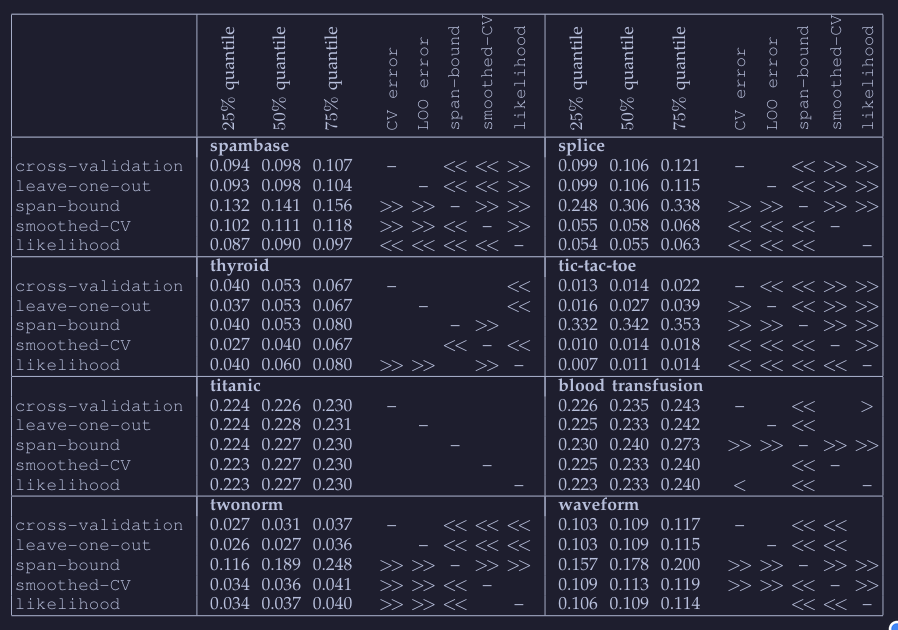
\includegraphics[width=0.8\textwidth]{winner.png}
		\caption{Результаты первых 20 эксперементов}
	\end{figure}



\end{frame}


\begin{frame}
	\frametitle{Результаты. Таблицы (2)}
	\begin{figure}
		\centering
		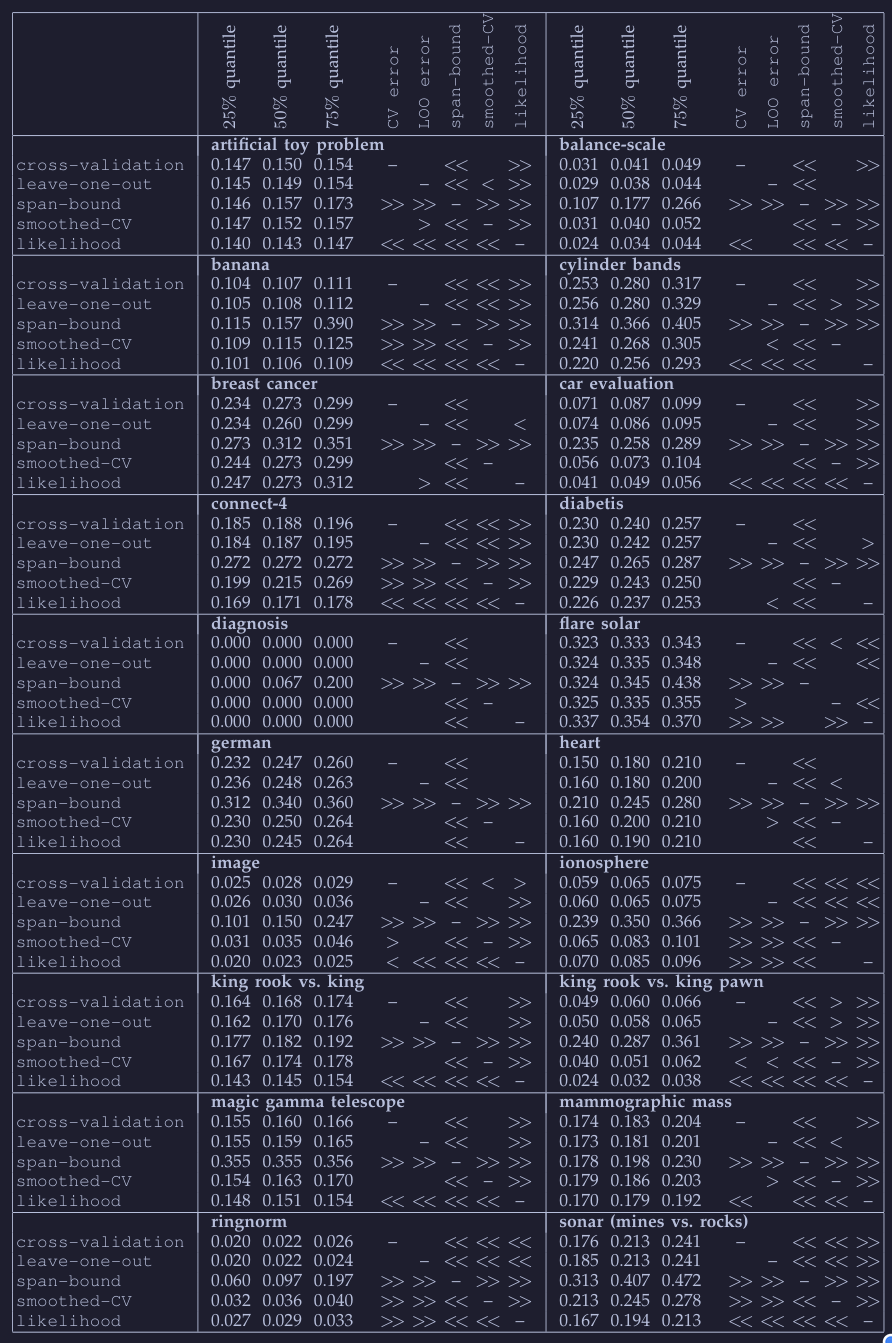
\includegraphics[height=0.8\textheight]{winner-true.png}
		\caption{Результаты остальных 8 эксперементов}
	\end{figure}

\end{frame}

\end{document}
